\documentclass{standalone}

\usepackage{tikz}
\usepackage{pgfplots}

\usetikzlibrary{calc}

\begin{document}
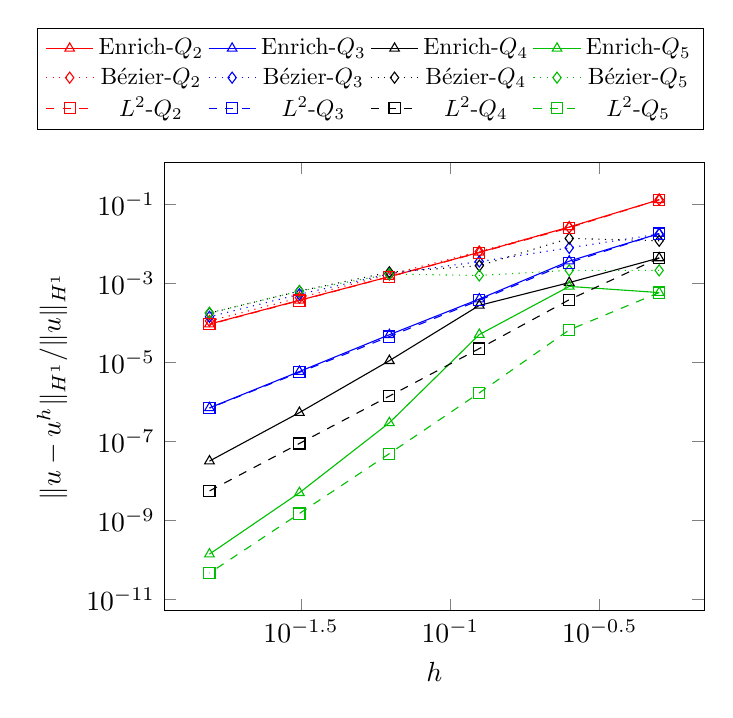
\begin{tikzpicture}
    \begin{loglogaxis}[
        legend columns=4,
    	legend style={at={(1,1.3)}, nodes={scale=.85, transform shape}},
        xlabel=$h$,
        ylabel=${\|u-u^{h}\|_{H^1}}/{\|u\|_{H^1}}$ 
    ]

    \addplot [color=red,mark=triangle] plot coordinates {

        (.5,        0.129375)
        (.25,       0.026405)
        (.125,      0.00603658)
        (.0625,     0.00146782)
        (0.03125,   0.0003708)
        (0.015625,  9.25896e-05)
    };

    
    \addplot [color=blue,mark=triangle] plot coordinates {

        (.5,        0.0180672)
        (.25,       0.00362157)
        (.125,      0.000398108)
        (.0625,     4.99073e-05)
        (0.03125,   5.85379e-06)
        (0.015625,  7.06388e-07)
    };

    \addplot [color=black,mark=triangle] plot coordinates {

        (.5,        0.00436143)
        (.25,       0.00103799)
        (.125,      0.00027525)
        (.0625,     1.10133e-05)
        (0.03125,   5.36393e-07)
        (0.015625,  3.18842e-08)
    };

    \addplot [color=green!75!black,mark=triangle] plot coordinates {


        (.5,        0.000581322)
        (.25,       0.000831278)
        (.125,      5.04533e-05)
        (.0625,     2.96255e-07)
        (0.03125,   5.03893e-09)
        (0.015625,  1.41627e-10)
    };

    
    \addplot [color=red,mark=diamond, every mark/.append style={solid}, dotted] plot coordinates {

        (.5,        0.130857)
        (.25,       0.0257758)
        (.125,      0.00636547)
        (.0625,     0.00165869)
        (0.03125,   0.000429584)
        (0.015625,  0.000111102)
    };

    
    \addplot [color=blue,mark=diamond, every mark/.append style={solid}, dotted] plot coordinates {

        (.5,        0.0176491)
        (.25,       0.00783653)
        (.125,      0.00353538)
        (.0625,     0.00172382)
        (0.03125,   0.000524267)
        (0.015625,  0.000142069)
    };

    \addplot [color=black,mark=diamond, every mark/.append style={solid}, dotted] plot coordinates {

        (.5,        0.0118698)
        (.25,       0.0135906)
        (.125,      0.00278118)
        (.0625,     0.00189586)
        (0.03125,   0.000634034)
        (0.015625,  0.000175352)
    };

    \addplot [color=green!75!black,mark=diamond, every mark/.append style={solid}, dotted] plot coordinates {


        (.5,        0.00211597)
        (.25,       0.00211906)
        (.125,      0.00157521)
        (.0625,     0.0017011)
        (0.03125,   0.000631516)
        (0.015625,  0.000177923)
    };


    \addplot [color=red,mark=square, every mark/.append style={solid}, dashed] plot coordinates {

        (.5,        0.129375)
        (.25,       0.0252897)
        (.125,      0.00594567)
        (.0625,     0.00146361)
        (0.03125,   0.000364493)
        (0.015625,  9.10358e-05)
    };

    
    \addplot [color=blue,mark=square, every mark/.append style={solid}, dashed] plot coordinates {

        (.5,        0.0180672)
        (.25,       0.00330952)
        (.125,      0.000371355)
        (.0625,     4.4961e-05)
        (0.03125,   5.57483e-06)
        (0.015625,  6.95478e-07)
    };

    \addplot [color=black,mark=square, every mark/.append style={solid}, dashed] plot coordinates {

        (.5,        0.00436143)
        (.25,       0.000383202)
        (.125,      2.23018e-05)
        (.0625,     1.40061e-06)
        (0.03125,   8.8722e-08)
        (0.015625,   5.5991e-09)
    };

    \addplot [color=green!75!black,mark=square, every mark/.append style={solid}, dashed] plot coordinates {


        (.5,        0.000581322)
        (.25,       6.60681e-05)
        (.125,      1.68549e-06)
        (.0625,     4.90895e-08)
        (0.03125,   1.50513e-09)
        (0.015625,  4.68227e-11)
    };


    \logLogSlopeTriangle{0.16}{0.075}{0.06}{5}{green!75!black};
    \logLogSlopeTriangle{0.16}{0.075}{0.245}{4}{black};
    \logLogSlopeTriangle{0.16}{0.075}{0.43}{3}{blue};
    \logLogSlopeTriangle{0.16}{0.075}{0.62}{2}{red};

    \legend{Enrich-$Q_2$\\Enrich-$Q_3$\\Enrich-$Q_4$\\Enrich-$Q_5$\\B\'ezier-$Q_2$\\B\'ezier-$Q_3$\\B\'ezier-$Q_4$\\B\'ezier-$Q_5$\\$L^2$-$Q_2$\\$L^2$-$Q_3$\\$L^2$-$Q_4$\\$L^2$-$Q_5$\\}
    \end{loglogaxis}
\end{tikzpicture}

\end{document}
